\documentclass[a4paper,11pt]{article}

% Packages essentiels
\usepackage[utf8]{inputenc}
\usepackage[T1]{fontenc}
\usepackage[numbers]{natbib}
\usepackage[french]{babel}
\usepackage{csquotes}
\usepackage{xcolor}
\usepackage{graphicx}
\usepackage{tabularx}
\usepackage{booktabs}
\usepackage{amsmath,amssymb,amsfonts}
\usepackage{float}
\usepackage{listings}
\usepackage{tcolorbox}
\usepackage{pgfplots}
\usepackage{parskip}
\usepackage[french]{datetime2}
\usepackage{multirow}
\usepackage{siunitx}
\usepackage{mdframed}
\usepackage[colorlinks=true]{hyperref}
\usepackage[nameinlink]{cleveref}
\usepackage{fontawesome5}
\usepackage{adjustbox} % Utilisé pour le logo Hugging Face

% Configuration de pgfplots
\pgfplotsset{compat=newest,compat/show suggested version=false}

% Configuration des boîtes de texte
\newmdenv[
    linewidth=1pt,
    topline=true,
    bottomline=true,
    leftline=true,
    rightline=true,
    backgroundcolor=gray!5,
    innertopmargin=10pt,
    innerbottommargin=10pt,
    innerrightmargin=10pt,
    innerleftmargin=10pt,
    skipabove=15pt,
    skipbelow=15pt
]{solution}

% Configuration pour le code Python
\lstset{
    language=Python,
    basicstyle=\ttfamily\small,
    frame=single,
    breaklines=true,
    keywordstyle=\color{blue},
    commentstyle=\color{green!60!black},
    stringstyle=\color{red},
    showstringspaces=false,
    backgroundcolor=\color{gray!5},
    literate={é}{{\'e}}1 {è}{{\`e}}1 {à}{{\`a}}1 {É}{{\'E}}1 {ù}{{\'u}}1
    {π}{{$\pi$}}1
    {≤}{{$\leq$}}1
    {≥}{{$\geq$}}1
    {≠}{{$\neq$}}1
    {²}{{$^2$}}1
    {⁸}{{$^8$}}1
    {⁷}{{$^7$}}1
    {⁶}{{$^6$}}1
    {⁵}{{$^5$}}1
    {⁴}{{$^4$}}1
    {³}{{$^3$}}1
}

% Configuration des marges
\usepackage[top=2cm, bottom=2cm, left=2.5cm, right=2.5cm]{geometry}

% Définition des environnements personnalisés
\newtcolorbox{graysection}[1]{
    colback=gray!10,
    colframe=white,
    title=#1,
    fonttitle=\bfseries\large,
    boxrule=0pt,
    arc=0pt,
    boxsep=5pt,
    left=10pt,right=10pt,top=10pt,bottom=10pt
}

% Commande TODO professionnelle
\newcommand{\todo}[1]{\textcolor{red}{\bfseries [TODO: #1]}}

% Informations du document
\newcommand{\titre}{
Agent conversationnel pour l'interrogation de la base de données Open Food Facts \\
\vspace{1cm} Description et planification du projet}
\newcommand{\auteurs}{Alain Boisvert}
\newcommand{\matricules}{994 029 313}
\newcommand{\destinataire}{Luc Lamontagne}
\newcommand{\cours}{IFT-6005 - Projet intégrateur}
\newcommand{\dateremise}{28 janvier 2025}

\title{IFT-6005 - Projet intégrateur - H25 \\ ~ \\ Agent conversationnel pour l'interrogation de la base de données Open Food Facts}
\author{Alain Boisvert}
\date{23 janvier 2025}

\begin{document}

\thispagestyle{empty}  % Pour éviter d'avoir un en-tête et un pied de page sur la page couverture

\includegraphics[width=5cm]{./figures/logo.jpg}	 % Pour inclure le logo de l'Université Laval
\vspace{4cm}  % Espacement vertical
\begin{center}	% On centre le texte
    \setlength{\baselineskip}{2.0\baselineskip}  % Multiplie l'interligne par 1.5
{\LARGE \bf \titre} \\  % \huge fait que le texte est gros, \bf fait que le texte est gras
\vspace{4cm}
\large Travail présenté à \destinataire \\ \vspace{0.3cm} \cours\\
\vspace{4cm}
% réalisé par \\ \auteurs ;\\ \matricules
{\large réalisé par \\ \vspace{0.3cm} \auteurs \\  \vspace{0.3cm} \matricules}
\vfill	% On va jusqu'au bas de la page avant de mettre le texte ci-dessous
{\large \dateremise} 
\pagebreak
\end{center}

\newpage
% \maketitle

%----------------------------------------------------------------------------------------
\section{Description du problème}  
\label{sec:probleme}

L'accès aux bases de données relationnelles repose traditionnellement sur des langages de requête structurés (par exemple, SQL),
excluant ainsi les utilisateurs dépourvus de compétences techniques. Cette contrainte limite l'exploitation optimale des
données, particulièrement dans les domaines nécessitant une accessibilité grand public.

Un cas d'usage illustratif est la consultation d'informations nutritionnelles. Des plateformes comme \textit{Open Food Facts}\footnote{\url{https://world.openfoodfacts.org/}}
agrègent des millions de fiches produits détaillées (composition, apports nutritifs, certifications), mais leur
interface requiert des requêtes manuelles ou des filtres prédéfinis. Pour un consommateur souhaitant poser des questions
plus complexes (\textit{\enquote{Quels en-cas sans allergènes ont un Nutri-score A ?}}), l'expérience utilisateur reste laborieuse.

Ce projet explore l'utilisation des grands modèles de langage (LLM) pour faciliter l'accès aux bases de données.
Les LLM peuvent comprendre les questions posées en langage naturel et les convertir en requêtes de base de données. Cette approche présente deux avantages majeurs :


\begin{itemize}
\item \textbf{Simplification de l'accès aux données :} Les utilisateurs peuvent poser des questions dans leur langage habituel, sans connaissances techniques.
\item \textbf{Amélioration de la qualité des réponses :} En accédant directement aux sources de données structurées, le système peut fournir des réponses plus précises et fiables.
\end{itemize}

L'objectif de ce projet est de développer un agent conversationnel capable de répondre à des questions en langage naturel en interrogeant la base de données de produits alimentaires
d'Open Food Facts.

%----------------------------------------------------------------------------------------
\section{Revue de littérature}
\label{sec:revue}

L'interaction en langage naturel avec les bases de données représente un défi majeur en intelligence artificielle. Les récents progrès des LLM ouvrent de nouvelles perspectives pour permettre aux utilisateurs de formuler des requêtes complexes sans connaître le langage SQL. Cette \enquote{très brève} 
revue de littérature examine les avancées récentes dans ce domaine, en se concentrant particulièrement sur les systèmes de conversion texte-vers-SQL utilisant des LLM.

\begin{itemize}
    \item L'étude de \citet{hong2024next} présente une revue complète de la conversion texte-vers-SQL basée sur les LLM et des défis techniques. Les auteurs présentent 
    une analyse des avancées récentes dans la conversion texte-vers-SQL basée sur les LLM.
    Les auteurs 
    fournissent également une introduction détaillée aux jeux de données
    et aux métriques conçus pour évaluer les systèmes de conversion texte-vers-SQL. 

    \item \citet{mohammadjafari2024natural} examinent l'évolution des systèmes de conversion texte-vers-SQL, 
    depuis les premiers modèles basés sur des règles jusqu'aux approches avancées utilisant les LLM, les jeux de test, les méthodes d'évaluation et les métriques d'évaluation. 
    Ils discutent des techniques de fine-tuning, d'apprentissage zero-shot et few-shot, et de l'augmentation des données.
    Ils étudient aussi le rôle de l'intégration des graphes de connaissances pour améliorer la précision contextuelle et la liaison des schémas dans ces systèmes. 

    \item \citet{zhu2024large} classifient les approches de conversion texte-vers-SQL basées sur les LLM en groupes selon leurs stratégies d'entraînement : ingénierie des prompts, fine-tuning, pré-entraînement et agents. Ils présentent également un résumé complet des jeux de données et des métriques d'évaluation. 
    
    \item \citet{gao2023text} proposent DAIL-SQL, une méthode d'ingénierie des prompts pour améliorer la conversion de textes vers SQL basée sur les LLM. 
    Les auteurs étudient l'ingénierie des prompts, incluant la représentation des questions, la sélection et l'organisation des exemples. 
    Leur méthode atteint une précision remarquable de 86,6\% sur le jeu de test Spider, démontrant qu'une ingénierie des promts peut significativement améliorer la qualité des requêtes SQL générées. Ils explorent également le potentiel des LLM open source dans la conversion texte-vers-SQL et le fine-tuning supervisé pour améliorer les performances. 

    \item \citet{biswal2024text2sql} présentent TAG (\textit{Table-Augmented Generation}, génération augmentée par table), une nouvelle approche pour interroger les bases de données en langage naturel. Ce modèle en trois étapes (synthèse de requêtes, exécution et génération de réponses) combine les capacités de raisonnement sémantique des LLM avec la puissance des systèmes de bases de données. 
    Cette approche permet de traiter des questions plus complexes nécessitant une combinaison de raisonnement textuel, de calculs et de connaissances générales.
    TAG surmonte les limitations des approches existantes comme Text2SQL et RAG (\textit{Retrieval-Augmented Generation}), offrant une amélioration de performance de 20-65\% dans les tests. 

    \item \citet{li2024can} introduisent le jeu de test BIRD, conçu pour répondre aux limitations des jeux de test de conversion texte-vers-SQL existants (comme Spider et WikiSQL). 
    BIRD contient 12~751~paires texte-vers-SQL et 95~bases de données d'une taille totale de 33,4~Go, couvrant 37~domaines professionnels. 
    Les auteurs se concentrent sur les défis liés aux données bruitées, aux connaissances externes et à l'efficacité SQL. 
    Les résultats montrent que même des LLM avancés comme GPT-4 n'atteignent que 54,89\% de précision d'exécution sur BIRD, significativement inférieur à la performance humaine (92,96\%).

    \item \citet{malekpour2024towards}, de Polytechnique Montréal, proposent une approche de routage LLM pour la conversion texte-vers-SQL, qui sélectionne dynamiquement le LLM le plus rentable capable de générer du SQL précis pour chaque requête. Ils présentent deux stratégies de routage (basées sur le score et sur la classification) qui atteignent une précision comparable au LLM le plus performant tout en réduisant les coûts, facilitant l'entraînement et permettant une inférence efficace.
\end{itemize}

Ces articles démontrent l'évolution rapide de la conversion texte-vers-SQL utilisant les LLM. 
Ils mettent en évidence l'importance des jeux de test, d'une ingénierie des prompts, et des approches innovantes 
pour rendre des systèmes plus performants.

Ces travaux sont pertinents pour notre projet d'agent conversationnel pour Open Food Facts. L'approche de DAIL-SQL pourrait être adaptée pour optimiser la conversion des questions nutritionnelles en requêtes SQL précises, tandis que l'approche TAG pourrait améliorer la qualité des réponses en combinant les données structurées avec le raisonnement sémantique. Les stratégies de routage LLM proposées par l'équipe de Polytechnique Montréal offrent des pistes pour optimiser les coûts. De plus, les méthodologies d'évaluation présentées dans ces articles, notamment dans le contexte de BIRD, pourront guider la création d'un jeu de test spécifique aux requêtes sur les produits alimentaires.

Ces travaux seront étudiés plus en détail au cours des prochaines semaines dans le cadre de ce projet afin d'identifier les meilleures pratiques à adopter.




% ----------------------------------------------------------------------------------------
\section{Approche proposée}
\label{sec:approche}


Le système proposé repose sur une architecture modulaire pour faciliter le développement, l'entraînement et l'évaluation, qui 
comprendra quatre composants clés interconnectés :

\begin{itemize}
    \item \textbf{Module de dialogue :} Responsable de maintenir le contexte conversationnel et de gérer les interactions avec l'utilisateur. 
    \item \textbf{Conversion texte-SQL :} Transforme les questions en langage naturel en requêtes SQL. 
    \item \textbf{Connecteur de base de données :} Interface avec une base de données pour l'exécution des requêtes.
    \item \textbf{Générateur de réponses :} Transforme les résultats bruts en réponses naturelles et contextuelles.
\end{itemize}

Nous débuterons par un LLM pré-entraîné pour le dialogue et capable d'utiliser des outils, 
probablement Qwen2-7B-Instruct\footnote{\url{https://huggingface.co/Qwen/Qwen2-7B-Instruct}} pour ses capacités natives de fonction calling.

La conversion texte-SQL sera réalisée en plusieurs étapes, inspirées de \citet{biswal2024text2sql}. Nous explorerons la 
possibilité d'utiliser du one-shot et few-shot learning pour améliorer la performance et un outil comme sqlglot\footnote{\url{https://github.com/tobymao/sqlglot}} 
pour valider la syntaxe des requêtes.

Pour la base de données, nous utiliserons une version simplifiée de la base de données Open Food Facts, stockée au format Parquet.
Ces données seront converties en une base DuckDB pour faciliter les requêtes SQL.

Pour les validations, nous utiliserons un ensemble de questions de référence, inspiré de BIRD mais spécifiquement créé pour les données d'Open Food Facts, pour évaluer la qualité des réponses.
Les métriques à considérer sont l'exactitude des réponses, le temps de réponse moyen, le taux de réussite multilingue et la robustesse aux données manquantes.

Je propose un développement incrémental, en commençant par une approche simple et évolutive vers un système plus complet.
Voici les étapes proposées :

\begin{itemize}
    \item Créer un système conversationnel avec un LLM open-source 
    \item Convertir les questions en requêtes SQL
    \item Créer un outil pour interroger la base de données via une requête SQL
    \item Générer une réponse à partir des résultats de la requête
    \item Évaluer la qualité des réponses et le temps d'exécution
    \item Optimiser le système pour améliorer les performances (par exemple, optimiser les prompts, faire du one-shot ou few-shot learning)
\end{itemize}

Cette approche modulaire permettra d'itérer rapidement tout en maintenant un haut niveau de fiabilité. Les choix technologiques restent volontairement flexibles pour s'adapter aux évolutions rapides du domaine des LLM.


%----------------------------------------------------------------------------------------
\section{Données utilisées}
\label{sec:donnees}

Une version simplifiée des données Open Food Facts au format Parquet est disponible sur~\adjustimage{height=1.3em,valign=c,raise=0.35ex}{figures/hf-logo.png}\,Hugging 
Face\footnote{\url{https://huggingface.co/datasets/openfoodfacts/product-database}}. 
Ce format orienté colonnes est particulièrement efficace pour le stockage et l'analyse de grands jeux de données sur un ordinateur personnel avec une RAM limitée.

La base complète contient 3~601~655 produits alimentaires décrits par 109 colonnes, incluant :

\begin{itemize}
    \item Informations générales : code-barres, nom, marque, quantité
    \item Nutrition : nutriments, vitamines, minéraux
    \item Composition : ingrédients, allergènes, additifs
    \item Certifications : labels (bio, sans gluten), scores (Nutri-score, NOVA, Eco-score, Green-Score)
    \item Origine et distribution : pays de fabrication, lieux de vente
\end{itemize}

Les données se présentent sous différents formats (listes, chaînes de caractères, nombres) avec une proportion importante de valeurs manquantes - jusqu'à 75\% pour certaines colonnes. Par exemple, l'Eco-score est absent dans 80\% des entrées.

La figure~\ref{fig:missing-values} présente la distribution de la complétude des colonnes de la base de données. On observe une distribution bimodale avec un grand nombre de colonnes très complètes (>95\%) et un second groupe de colonnes peu renseignées (<30\%).

\begin{figure}[htbp]
    \centering
    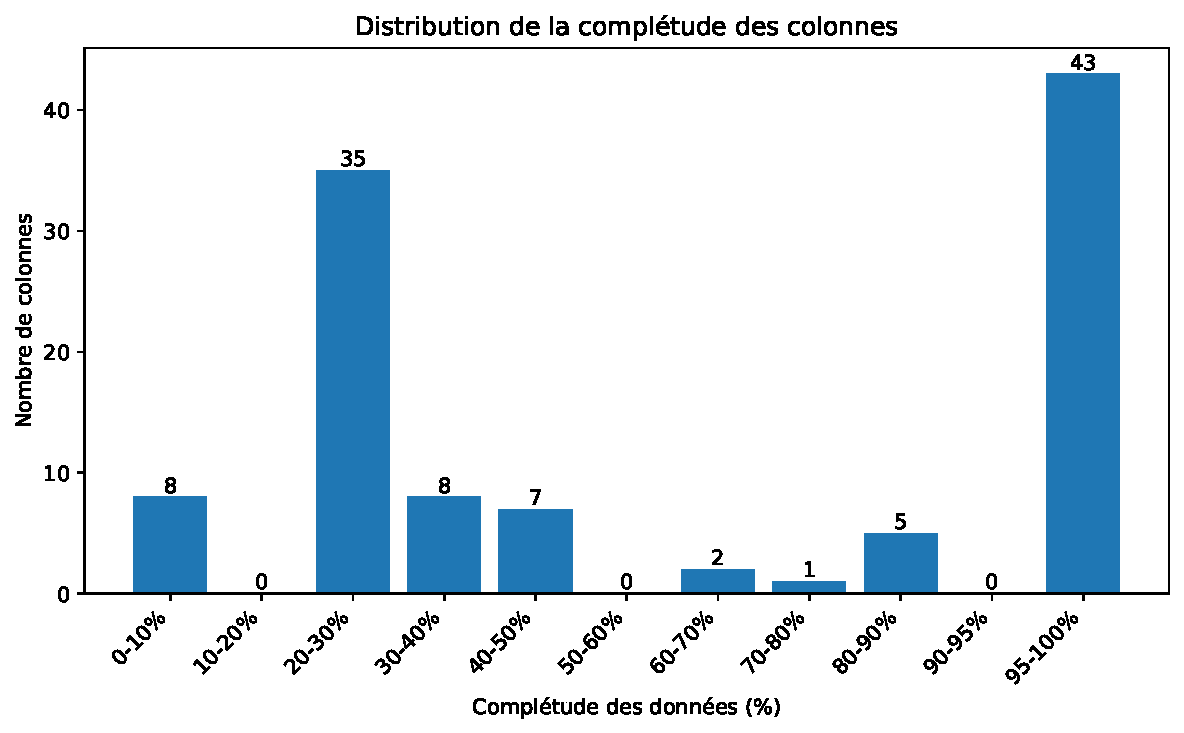
\includegraphics[width=0.9\textwidth]{figures/missing_values.pdf}
    \caption{Distribution de la complétude des colonnes de la base de données}
    \label{fig:missing-values}
\end{figure}

Pour ce projet, nous utiliserons un sous-ensemble de 94~802 produits alimentaires canadiens afin d'optimiser les temps de traitement.

%----------------------------------------------------------------------------------------
\section{Évaluation du système}
\label{sec:evaluation}

L'évaluation du système s'appuiera sur trois métriques principales, inspirées des articles cités précédemment, tout en étant adaptées aux spécificités des données nutritionnelles :

\begin{enumerate}
   \item \textbf{Précision d'exécution (EX)} : Cette métrique, adoptée dans la littérature récente \citep{li2024can}, 
évalue si les requêtes SQL générées produisent les résultats attendus. Pour notre cas d'usage, nous créerons un jeu 
de test de 100 questions nutritionnelles courantes avec leurs requêtes SQL de référence et les résultats attendus formatés. 
Cette standardisation des résultats de référence est nécessaire pour une comparaison objective et automatisée. La précision 
sera calculée en comparant les résultats d'exécution des requêtes générées avec ceux des requêtes de référence, plutôt 
qu'en comparant directement le code SQL. Cette approche permet d'accepter des formulations SQL différentes tant qu'elles 
produisent les mêmes résultats.

   \item \textbf{Taux de couverture des données manquantes (TCM)} : Cette métrique évalue la capacité du système à fournir des réponses pertinentes malgré l'absence de certaines données. Trois stratégies sont employées :
   \begin{itemize}
       \item Utilisation d'attributs alternatifs : par exemple, estimer le Nutri-Score à partir des valeurs nutritionnelles
       \item Reformulation des requêtes pour exploiter les données disponibles
       \item Communication claire des limitations et du niveau de confiance des réponses
   \end{itemize}
   Le TCM sera évalué sur le même jeu de test de 100 questions, en calculant le pourcentage de cas où le système parvient 
   à fournir une réponse exploitable malgré des données manquantes. Une réponse est considérée exploitable si elle utilise 
   avec succès au moins une des trois stratégies mentionnées. Cette approche permet d'optimiser l'utilité des réponses 
   même avec une base de données incomplète.

   \item \textbf{Temps de réponse moyen (TRM)} : Cette métrique mesure le temps total nécessaire pour traiter une requête, depuis la réception de la question en langage naturel jusqu'à la génération de la réponse finale. Elle inclut :
   \begin{itemize}
       \item Le temps de conversion de la question en SQL
       \item Le temps d'exécution de la requête sur la base de données
       \item Le temps de génération de la réponse en langage naturel
   \end{itemize}
   Le TRM sera mesuré sur une configuration matérielle standardisée pour assurer la comparabilité des résultats au fil 
   du développement. Cette métrique est particulièrement importante pour évaluer l'utilisabilité du système dans un 
   contexte réel.
\end{enumerate}

Ces métriques seront évaluées sur différentes catégories de questions (simples, complexes, multiples critères) pour assurer une évaluation complète du système. 

Ces tests d'évaluation seront intégrés tout au long du développement pour guider les améliorations du système.


%----------------------------------------------------------------------------------------
\section{Tâches à faire}
\label{sec:taches}

Cette planification de projet (230h) suit une approche incrémentale, permettant de développer et tester chaque composant de manière itérative :

\begin{enumerate}
    \item \textbf{Préparation et configuration (30h)}
    \begin{itemize}
        \item Mise en place de l'environnement de développement (5h)
        \item Préparation de la base de données Open Food Facts canadienne (5h)
        \item Créer un jeu de test de 100 questions de référence (10h)
        \item Implémentation des scripts d'évaluation des trois métriques (10h)
    \end{itemize}

    \item \textbf{Développement du système de base (75h)}
    \begin{itemize}
        \item Implémentation du module de dialogue avec Qwen2-7B-Instruct (20h)
        \item Développement de la conversion texte-SQL de base (25h)
        \item Création du connecteur de base de données DuckDB (5h)
        \item Implémentation du générateur de réponses simples (25h)
    \end{itemize}

    \item \textbf{Rapport de mi-session (25h)}
    \begin{itemize}
        \item Analyse des résultats (10h)
        \item Rédaction du rapport de mi-session (15h)
    \end{itemize}

    \item \textbf{Optimisations et fonctionnalités avancées (55h)}
    \begin{itemize}
        \item Amélioration de la gestion des données manquantes (15h)
        \item Implémentation du one-shot et few-shot learning (20h)
        \item Optimisation des prompts et des requêtes SQL (20h)
    \end{itemize}

    \item \textbf{Documentation et finalisation (25h)}
    \begin{itemize}
        \item Rédaction du rapport final (15h)
        \item Préparation de la présentation orale (5h)
        \item Netoyage du code et de la documentation du dépôt GitHub (5h)
    \end{itemize}
\end{enumerate}

Cette planification inclut des jalons de validation à chaque étape majeure pour s'assurer que le développement reste 
aligné avec les objectifs du projet. Les heures allouées tiennent compte des défis potentiels liés à l'intégration 
des composants et à la gestion des données incomplètes d'Open Food Facts.


% Section Bibliographie
\label{sec:biblio}
\bibliographystyle{plainnat}
\bibliography{refs}  % Fichier .bib sans l'extension


\iffalse

Cette section en commentaires contient des exemples de code LaTeX pour les tableaux, les figures, les listes, etc.

Awesome-Text2SQL
https://github.com/eosphoros-ai/Awesome-Text2SQL


# Exemple de tableau
\begin{tabularx}{\textwidth}{llX}
\toprule
\textbf{RAG} & \textbf{Agents} \\
\midrule
Accès précis aux données & Gestion du flux décisionnel \\
Maintien du contexte court & Coordination multi-étapes \\
\bottomrule
\end{tabularx}

# Exemple de tableau
\begin{table}[ht]
\centering
\caption{Exemple de données nutritionnelles}
\begin{tabular}{lrrr}
\toprule
Produit & Calories (kcal) & Protéines (g) & Sucre (g) \\
\midrule
Lait 2\% & 130 & 8 & 12 \\
Pain complet & 240 & 9 & 3 \\
Yaourt nature & 150 & 5 & 7 \\
\bottomrule
\end{tabular}
\end{table}

\fi

\end{document}